\section{Dataset Robustness: AllSidesV2 Random Split}
\label{sec:random-split-comparison}

The preceding sections estimated all causal effects on articles drawn from the AllSidesV2 media split. Because the media split groups articles by source outlet, a classifier trained on that split can exploit source-level regularities that are not present in the underlying ideological signal. To assess whether the causal patterns reported above generalize under source leakage, we repeat the community- and topic-level analyses on a $\num{4104}$-article subset of the AllSidesV2 random split test set. The community assignments are identical to those used in Section~\ref{sec:community-level-results}; only the article subset differs. We restrict the comparison to two annotation paradigms: Human annotations and the fine-tuned RoBERTa model reported as Best Full ($T_{id}(32){+}T_h$) in Table~\ref{tab:extended_main}, which reaches $\text{F1}_{\text{macro}} = 89.29$ on the random split. Sentiment annotations are held constant across splits, so any divergence between the Human and Fine-tuned RoBERTa ATEs isolates the effect of ideology-label provenance.

If source leakage fully explains Fine-tuned RoBERTa's causal divergence from Human on the media split, then removing source leakage via the random split should tighten Human-vs-classifier alignment at both the community and topic levels. Persistence of directional disagreement or the appearance of new sign flips under the random split would instead falsify that hypothesis and indicate that the residual divergence originates from features of the text that the sentiment-and-community representation does not capture.

\subsection{Community-Level Results}
\label{sec:random-community-level-results}

\begin{figure}[h!]
    \centering
    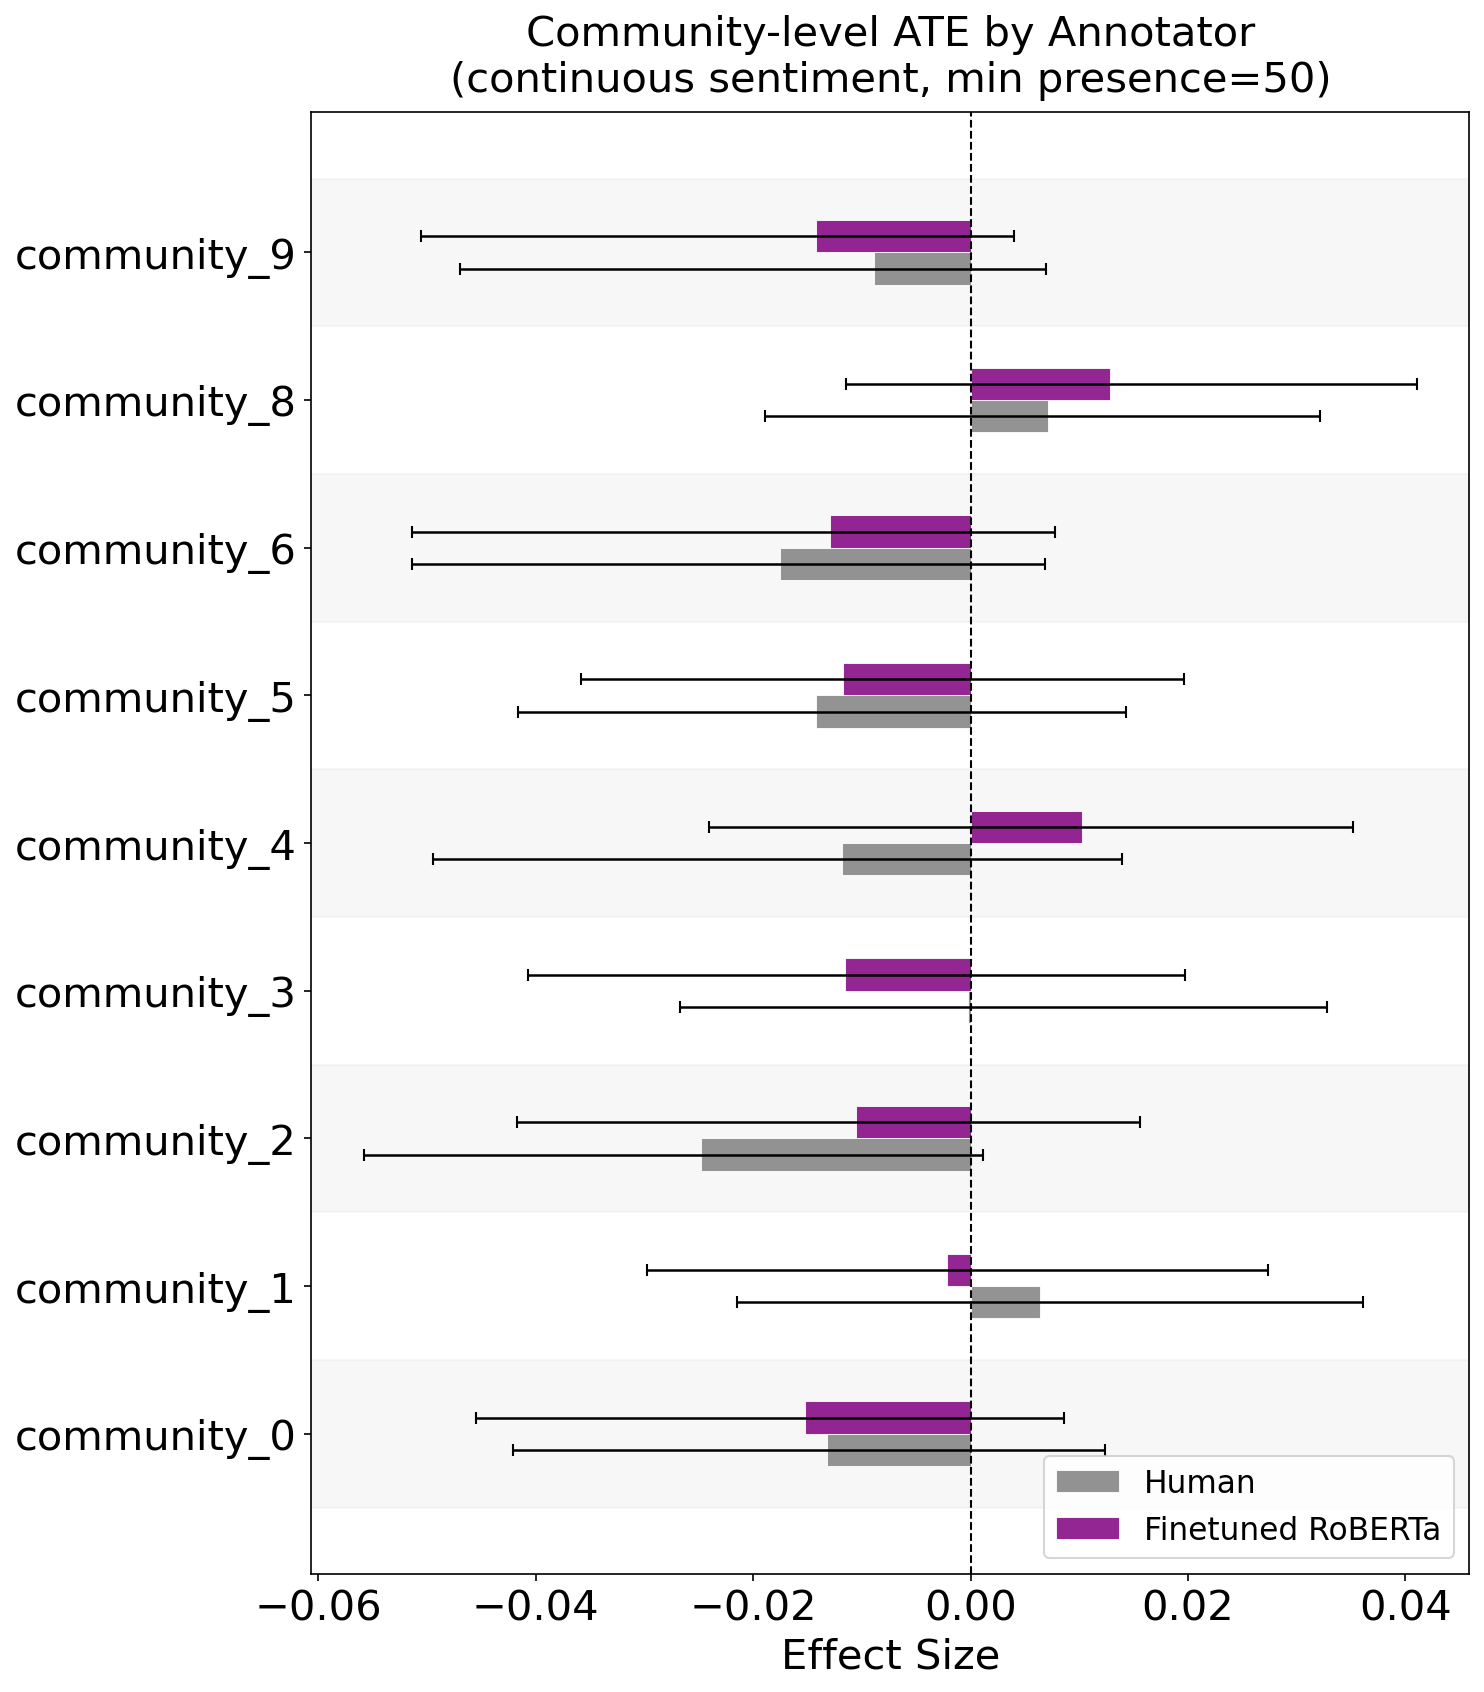
\includegraphics[width=0.7\textwidth]{sections/images/causal_analysis/random_split/ate_communities.png}
    \caption{Community-level ATE (continuous sentiment) under the AllSidesV2 random split. Human and Fine-tuned RoBERTa paradigms shown for the nine communities passing the minimum presence threshold of 50 articles.}
    \label{fig:random_community_ate}
\end{figure}

No community reaches significance under either paradigm on the random split. This is consistent with the reduced sample size relative to the media-split analysis ($\num{4104}$ versus the larger corpus used in Section~\ref{sec:community-level-results}), which mechanically widens confidence intervals. Point estimates nevertheless reveal two notable divergences between Human and Fine-tuned RoBERTa annotations that are not observable under the media split. Table~\ref{tab:random-community-delta} contrasts Community~1 (Elections and Campaigns) and Community~4 (Culture and Education) across both splits. The full community-level breakdown for the random split is reported in Appendix~\ref{sec:appendix-random-split}, Table~\ref{tab:random-community-ate-full}.

\begin{table}[ht]
  \centering
  \small
  \begin{tabular}{l c l l}
    \toprule
    \textbf{Community} & \textbf{N} & \textbf{Human (CI)} & \textbf{FT RoBERTa (CI)} \\
    \midrule
    \multicolumn{4}{l}{\textit{AllSidesV2 media split}} \\
    Comm.\ 1 (Elections/Campaigns) & \num{3628} & $+0.016\ [-0.002,\ +0.034]$ & $+0.011\ [-0.008,\ +0.028]$ \\
    Comm.\ 4 (Culture/Education)   & 720        & $+0.013\ [-0.014,\ +0.025]$ & $+0.007\ [-0.015,\ +0.019]$ \\
    \midrule
    \multicolumn{4}{l}{\textit{AllSidesV2 random split}} \\
    Comm.\ 1 (Elections/Campaigns) & \num{1551} & $+0.006\ [-0.022,\ +0.036]$ & $\mathbf{-0.002}\ [-0.030,\ +0.027]$ \\
    Comm.\ 4 (Culture/Education)   & 372        & $\mathbf{-0.012}\ [-0.049,\ +0.014]$ & $+0.010\ [-0.024,\ +0.035]$ \\
    \bottomrule
  \end{tabular}
  \caption{Community-level ATE comparison for Communities~1 and~4 across the AllSidesV2 media and random splits. \textbf{Bolded} point estimates mark sign reversals between the Human and Fine-tuned RoBERTa paradigms; both communities exhibit a sign flip on the random split that is absent under the media split. All confidence intervals cross zero, so no individual effect reaches 95\% significance.}
  \label{tab:random-community-delta}
\end{table}

Under the media split, the Human and Fine-tuned RoBERTa point estimates agree in direction for both communities (positive in each case). Under the random split, the paradigms disagree directionally: in Community~1 the Human estimate remains positive ($+0.006$) while the Fine-tuned RoBERTa estimate is slightly negative ($-0.002$); in Community~4 the Human estimate is negative ($-0.012$) while the Fine-tuned RoBERTa estimate is positive ($+0.010$). These sign flips do not survive significance testing, but their appearance in a comparison where sentiment annotations, community assignments, and article subset are all held constant is a direct indication that the ideology-label provenance alone can reorient the point estimate.

\subsubsection{Community-Level Mediation Analysis}
\label{sec:random-community-mediation-results}

For parity with Section~\ref{sec:community-mediation-results}, we decompose each community-level ATE into direct and indirect components using natural effect mediation on the four pathways among Communities~0, 1, and 2 under Human and Fine-tuned RoBERTa. All four pathways satisfy the minimum presence threshold of 50 articles on the random split ($N = \num{1551}$ for the $1 \to 0$ and $1 \to 2$ pathways, $N = \num{1022}$ for $0 \to 1$, and $N = 536$ for $2 \to 1$), so no pathway is skipped on sample-size grounds. No community reaches significance on the random split under either paradigm, so the decomposition is structurally less informative here than on the media split, but the direct-dominates-indirect pattern reported in Section~\ref{sec:community-mediation-results} remains testable.

Table~\ref{tab:random-community-mediation} reports the full decomposition under the $Q_{25} \to Q_{75}$ contrast. Three patterns emerge. First, the direct channel continues to dominate the indirect channel in every pathway and under both paradigms, mirroring the media-split finding. Second, none of the eight cells reach 95\% significance, consistent with the smaller per-pathway sample size under the random split and matching the non-significance observed at the community ATE level. Third, the Fine-tuned RoBERTa NIE on the $1 \to 0$ pathway flips sign relative to its media-split value ($+0.004 \to -0.000$), echoing the topic-level Trump-NIE sign flip reported in Section~\ref{sec:random-trump-mediation}. The $0 \to 1$ pathway is the only one on which both paradigms agree on a clearly negative NIE (Human $-0.017$, Fine-tuned RoBERTa $-0.019$), suggesting that on the random split the indirect $0 \to 1$ channel carries a small leftward push that the media-split decomposition did not surface. Mediation decomposition figures for the remaining three pathways ($0 \to 1$, $1 \to 2$, $2 \to 1$) are deferred to Appendix~\ref{sec:appendix-community-mediation}.

\begin{table}[h]
\centering
\footnotesize
\begin{tabular}{lcccccc}
\toprule
Annotator & TE & 95\% CI (TE) & NDE & 95\% CI (NDE) & NIE & 95\% CI (NIE) \\
\midrule
\multicolumn{7}{l}{\textit{Community $1 \to 0$ ($N=\num{1551}$, sentiment contrast $-0.3$ to $+0.1$)}} \\
\midrule
Human              & $+0.004$ & $[-0.082,\ +0.091]$ & $-0.006$ & $[-0.034,\ +0.033]$ & $+0.010$ & $[-0.005,\ +0.019]$ \\
Fine-tuned RoBERTa & $-0.007$ & $[-0.092,\ +0.078]$ & $-0.007$ & $[-0.041,\ +0.024]$ & $-0.000$ & $[-0.008,\ +0.016]$ \\
\midrule
\multicolumn{7}{l}{\textit{Community $1 \to 2$ ($N=\num{1551}$, sentiment contrast $-0.3$ to $+0.1$)}} \\
\midrule
Human              & $+0.001$ & $[-0.081,\ +0.083]$ & $-0.003$ & $[-0.034,\ +0.033]$ & $+0.004$ & $[-0.003,\ +0.011]$ \\
Fine-tuned RoBERTa & $-0.007$ & $[-0.088,\ +0.073]$ & $-0.007$ & $[-0.041,\ +0.024]$ & $-0.000$ & $[-0.005,\ +0.009]$ \\
\midrule
\multicolumn{7}{l}{\textit{Community $0 \to 1$ ($N=\num{1022}$, sentiment contrast $-0.2$ to $+0.1$)}} \\
\midrule
Human              & $-0.031$ & $[-0.143,\ +0.081]$ & $-0.014$ & $[-0.064,\ +0.022]$ & $-0.017$ & $[-0.033,\ +0.016]$ \\
Fine-tuned RoBERTa & $-0.040$ & $[-0.154,\ +0.074]$ & $-0.021$ & $[-0.069,\ +0.018]$ & $-0.019$ & $[-0.030,\ +0.018]$ \\
\midrule
\multicolumn{7}{l}{\textit{Community $2 \to 1$ ($N=536$, sentiment contrast $-0.2$ to $+0.1$)}} \\
\midrule
Human              & $-0.041$ & $[-0.141,\ +0.058]$ & $-0.055$ & $[-0.103,\ +0.007]$ & $+0.013$ & $[-0.020,\ +0.025]$ \\
Fine-tuned RoBERTa & $-0.013$ & $[-0.109,\ +0.084]$ & $-0.030$ & $[-0.078,\ +0.032]$ & $+0.017$ & $[-0.018,\ +0.035]$ \\
\bottomrule
\end{tabular}
\caption{Random-split community-level mediation results ($Q_{25} \to Q_{75}$ contrast) for Human and Fine-tuned RoBERTa paradigms. No cell reaches 95\% significance; all confidence intervals cross zero. The direct channel (NDE) dominates the indirect channel (NIE) in every pathway under both paradigms.}
\label{tab:random-community-mediation}
\end{table}

\begin{figure}[h!]
    \centering
    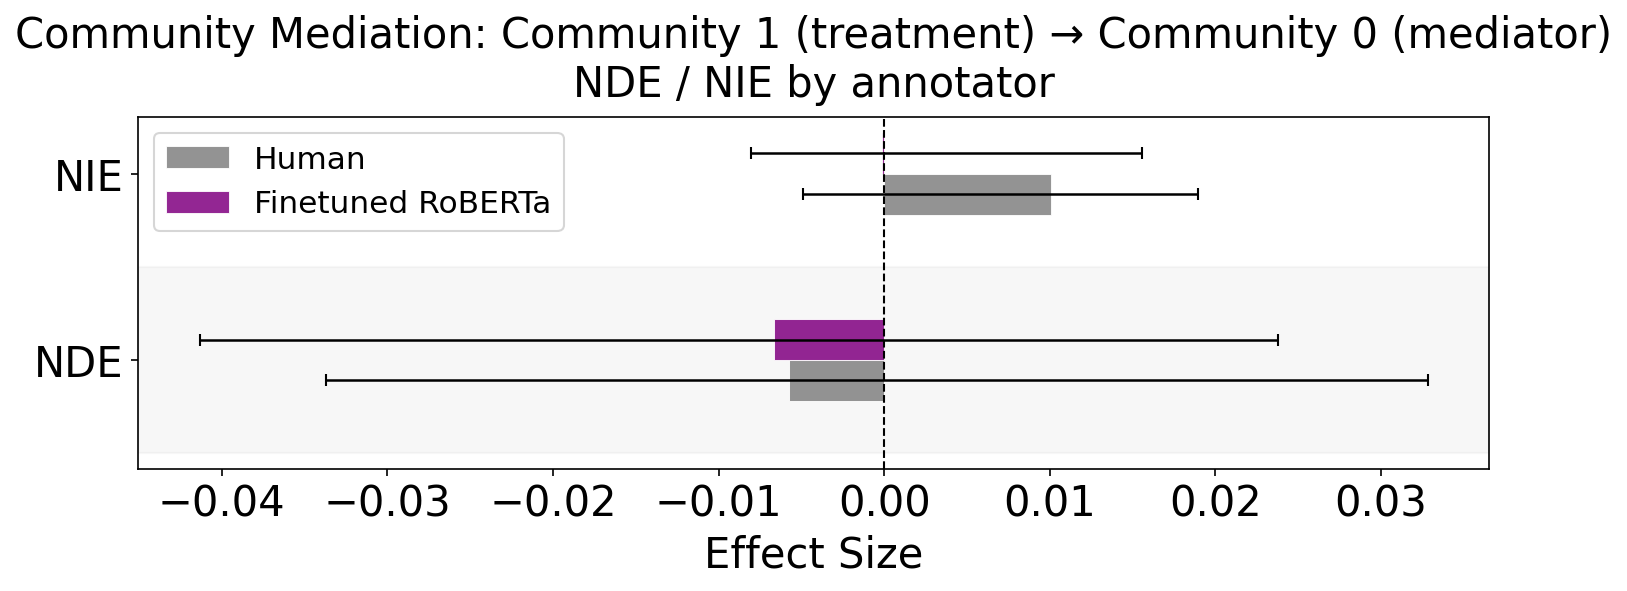
\includegraphics[width=0.7\textwidth]{sections/images/causal_analysis/random_split/mediation_community_1_0.png}
    \caption{Mediation decomposition for the Community $1 \to 0$ pathway under the AllSidesV2 random split ($N = \num{1551}$). Total Effect (TE), Natural Direct Effect (NDE), and Natural Indirect Effect (NIE) shown for the $Q_{25} \to Q_{75}$ contrast across Human and Fine-tuned RoBERTa paradigms. Decomposition figures for the remaining three pathways ($0 \to 1$, $1 \to 2$, $2 \to 1$) are reported in Appendix~\ref{sec:appendix-community-mediation}.}
    \label{fig:random-mediation-1-0}
\end{figure}

\subsection{Topic-Level Results}
\label{sec:random-topic-level-results}

\subsubsection{Multi-Treatment DML Results}
\label{sec:random-multi-treatment-results}

\begin{figure}[h!]
    \centering
    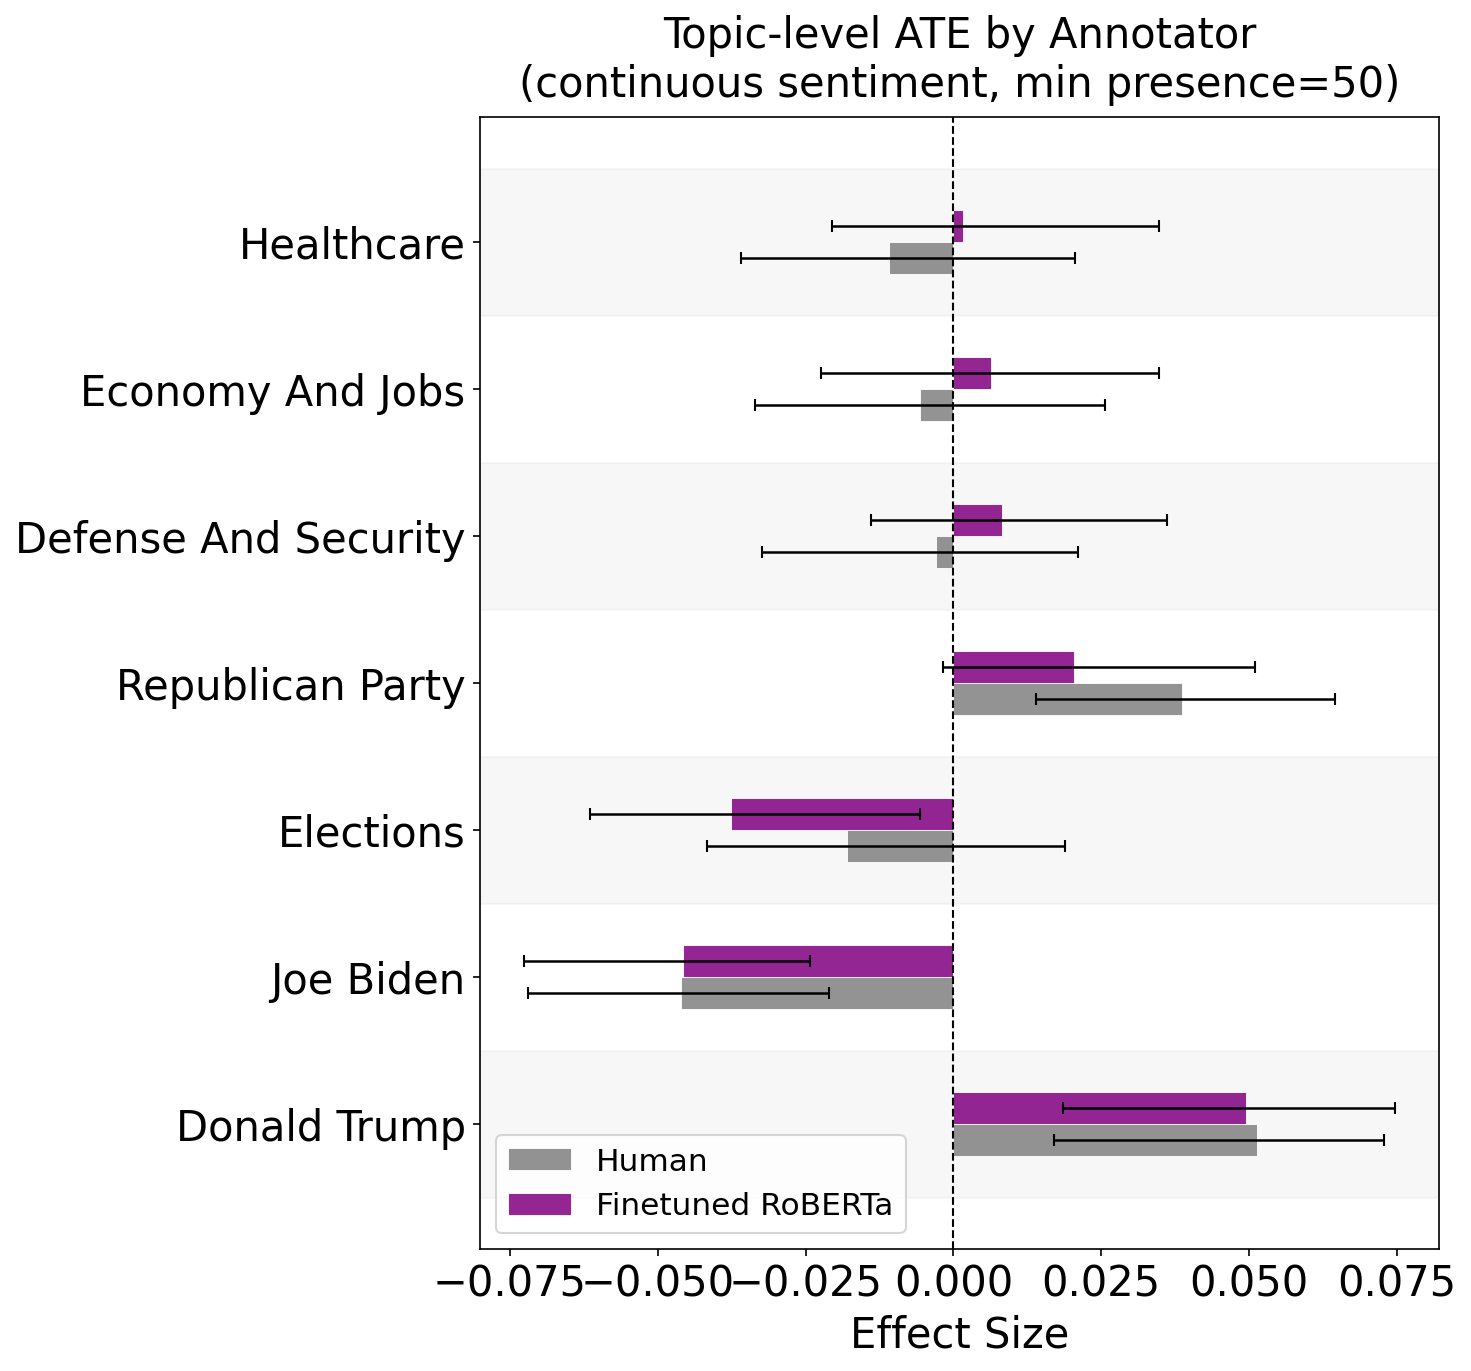
\includegraphics[width=0.7\textwidth]{sections/images/causal_analysis/random_split/ate_topics.png}
    \caption{Topic-level ATE (continuous sentiment) under the AllSidesV2 random split for the top 20 qualifying topics. Human and Fine-tuned RoBERTa paradigms shown with 95\% bootstrap confidence intervals.}
    \label{fig:random_topic_ate}
\end{figure}

Fewer topics reach significance under the random split than under the media split. Donald Trump remains the strongest and most robust effect under both splits and both paradigms, reaching significance in all four cells. Joe Biden's effect size increases substantially under the random split ($-0.0461$ Human, $-0.0458$ Fine-tuned RoBERTa), whereas under the media split the Human estimate narrowly missed significance ($-0.0143$). Republican Party retains significance under the Human paradigm in both splits, but loses significance for Fine-tuned RoBERTa under the random split (CI $[-0.002, +0.051]$). Elections exhibits the opposite pattern: it fails to reach significance under either paradigm on the media split, but the Fine-tuned RoBERTa estimate tightens to $-0.0375$ with a CI of $[-0.061, -0.006]$ on the random split, passing the significance threshold. Table~\ref{tab:random-topic-delta} summarizes the four topics across both splits. The full 20-topic random-split table with confidence intervals is reported in Appendix~\ref{sec:appendix-random-split}, Table~\ref{tab:random-multi-continuous-full}.

\begin{table}[ht]
  \centering
  \small
  \begin{tabular}{l c l l}
    \toprule
    \textbf{Topic} & \textbf{N} & \textbf{Human (CI)} & \textbf{FT RoBERTa (CI)} \\
    \midrule
    \multicolumn{4}{l}{\textit{AllSidesV2 media split}} \\
    Donald Trump     & \num{1424} & $\mathbf{+0.0427}\ [+0.025,\ +0.059]$ & $\mathbf{+0.0449}\ [+0.029,\ +0.062]$ \\
    Joe Biden        & 288        & $-0.0143\ [-0.032,\ +0.000]$ & $\mathbf{-0.0192^{*}}\ [-0.036,\ -0.002]$ \\
    Elections        & \num{1709} & $-0.0066\ [-0.023,\ +0.016]$ & $-0.0198\ [-0.038,\ +0.001]$ \\
    Republican Party & 293        & $\mathbf{+0.0367}\ [+0.023,\ +0.052]$ & $\mathbf{+0.0274}\ [+0.012,\ +0.043]$ \\
    \midrule
    \multicolumn{4}{l}{\textit{AllSidesV2 random split}} \\
    Donald Trump     & 572        & $\mathbf{+0.0513}\ [+0.017,\ +0.073]$ & $\mathbf{+0.0495}\ [+0.018,\ +0.075]$ \\
    Joe Biden        & 260        & $\mathbf{-0.0461}\ [-0.072,\ -0.021]$ & $\mathbf{-0.0458}\ [-0.073,\ -0.024]$ \\
    Elections        & 572        & $-0.0180\ [-0.042,\ +0.019]$ & $\mathbf{-0.0375}\ [-0.061,\ -0.006]$ \\
    Republican Party & 127        & $\mathbf{+0.0387}\ [+0.014,\ +0.065]$ & $+0.0204\ [-0.002,\ +0.051]$ \\
    \midrule
    \multicolumn{4}{l}{\textit{Delta (random $-$ media)}} \\
    Donald Trump     & --- & $+0.0086$ & $+0.0046$ \\
    Joe Biden        & --- & \textcolor{blue}{$-0.0318$} & \textcolor{blue}{$-0.0266$} \\
    Elections        & --- & \textcolor{blue}{$-0.0114$} & \textcolor{blue}{$-0.0177$} \\
    Republican Party & --- & $+0.0020$ & \textcolor{blue}{$-0.0070$} \\
    \bottomrule
  \end{tabular}
  \caption{Topic-level ATE comparison across the AllSidesV2 media and random splits for four representative topics. \textbf{Bolded} ATEs have CIs that exclude zero. The Delta section reports the per-paradigm difference between random-split and media-split point estimates; entries coloured \textcolor{blue}{blue} indicate that the random-split estimate is more leftward (more negative) than the media-split estimate.}
  \label{tab:random-topic-delta}
\end{table}

\subsubsection{Mediation Analysis Results}
\label{sec:random-trump-mediation}

\begin{figure}[h!]
    \centering
    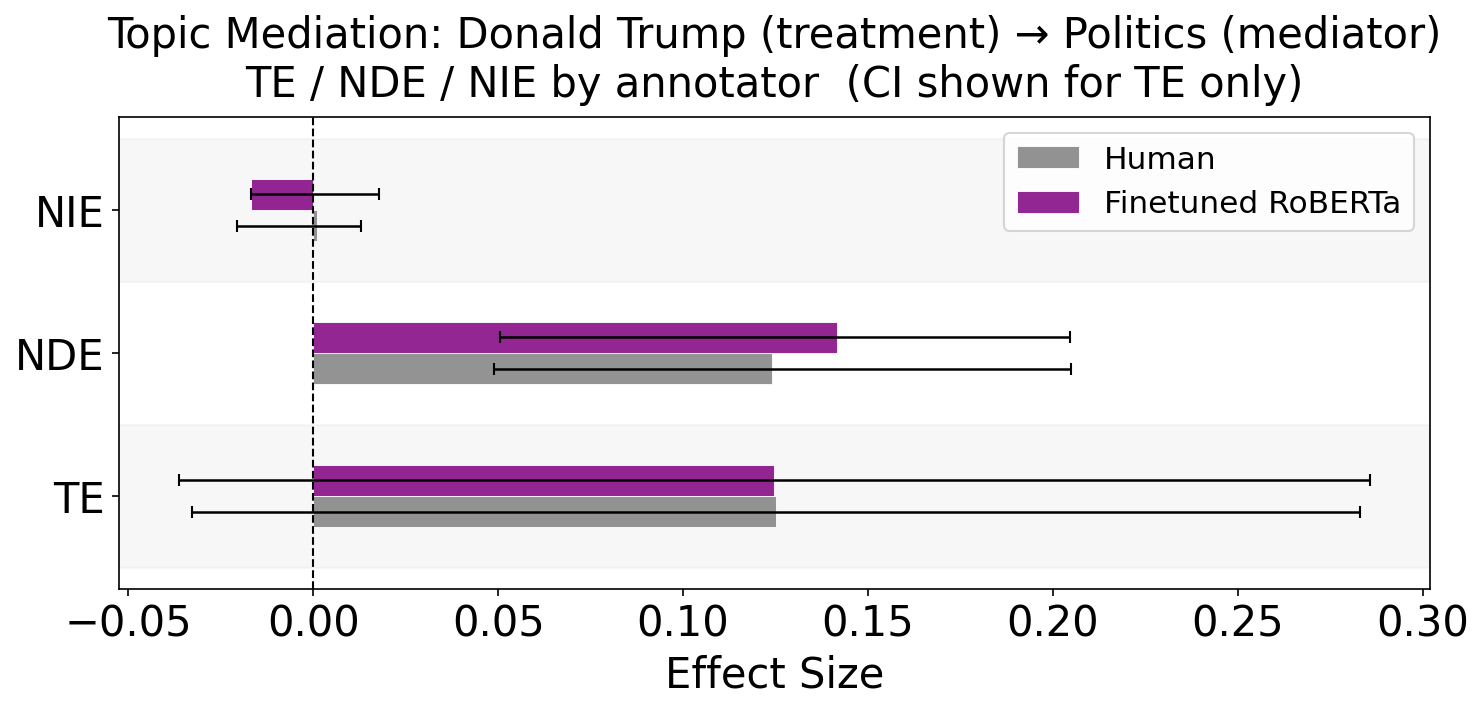
\includegraphics[width=0.7\textwidth]{sections/images/causal_analysis/random_split/mediation_topic_Donald_Trump_m_Politics.png}
    \caption{Mediation decomposition for Donald Trump sentiment as treatment and Politics sentiment as mediator under the AllSidesV2 random split ($N = 572$). Total Effect (TE), Natural Direct Effect (NDE), and Natural Indirect Effect (NIE) shown for the $Q_{25} \to Q_{75}$ contrast across Human and Fine-tuned RoBERTa paradigms.}
    \label{fig:random_trump_mediation}
\end{figure}

The media-split analysis (Section~\ref{sec:topic-mediation-results}, Table~\ref{tab:te-trump}) produced a borderline-significant Total Effect for Human annotations ($\widehat{\text{TE}} = +0.135$) and a significant Total Effect for Fine-tuned RoBERTa ($\widehat{\text{TE}} = +0.154^{*}$) on the $Q_{25} \to Q_{75}$ contrast. Under the random split, the Total Effect point estimates are nearly identical in magnitude ($+0.125$ for both Human and Fine-tuned RoBERTa on the $Q_{25} \to Q_{75}$ contrast), but neither reaches significance: the Human CI is $[-0.033, +0.283]$ and the Fine-tuned RoBERTa CI is $[-0.036, +0.286]$. The smaller subsample ($N = 572$ versus $N = \num{1424}$ for the media split) mechanically contributes to the wider intervals. The indirect channel, however, exhibits a structural change: the Fine-tuned RoBERTa Natural Indirect Effect flips sign, moving from $+0.019$ under the media split to $-0.017$ under the random split, while the Human NIE remains slightly positive in both splits ($+0.010$ media, $+0.001$ random). The direct channel (NDE) remains dominant and positive in all four cells. The full mediation decomposition for both percentile contrasts is reported in Appendix~\ref{sec:appendix-random-split}, Table~\ref{tab:random-te-trump-full}.

\subsubsection{Topic-Level Summary}
\label{sec:random-causal-summary-topic}

The media-split topic-level analysis (Section~\ref{sec:causal-summary-topic}) established a clear partisan pattern: topics associated with Democratic figures carry uniformly negative ATEs under both Human and Fine-tuned RoBERTa, while topics associated with Republican figures carry uniformly positive ATEs, with Donald Trump the most robust cross-paradigm effect. Under the random split, the headline partisan pattern survives: Donald Trump remains significant and positive under both paradigms; Joe Biden remains negative and in fact strengthens (from $-0.014$ to $-0.046$ for Human and from $-0.019$ to $-0.046$ for Fine-tuned RoBERTa); Democratic-versus-Republican directional agreement between Human and Fine-tuned RoBERTa is preserved on every topic that was significant under the media split. The pattern that does \emph{not} survive is paradigm-by-paradigm alignment on which topics reach significance: Republican Party, significant under both paradigms on the media split, loses significance under Fine-tuned RoBERTa on the random split; Elections, non-significant under either paradigm on the media split, becomes significant under Fine-tuned RoBERTa on the random split. The directional core is therefore robust to the split; the significance structure is not.

\subsection{Cross-Split Synthesis}
\label{sec:cross-split-synthesis}

Three concrete deviations separate the random-split results from the media-split results, and all three arise with sentiment annotations, community assignments, and article identities held constant across splits. At the community level, Communities~1 (Elections and Campaigns) and~4 (Culture and Education) both exhibit sign flips between Human and Fine-tuned RoBERTa point estimates on the random split that are absent under the media split (Table~\ref{tab:random-community-delta}). At the topic level, Elections gains significance under Fine-tuned RoBERTa while Republican Party loses it, and Joe Biden's effect magnitude roughly triples (Table~\ref{tab:random-topic-delta}). On the Donald Trump mediation, the Fine-tuned RoBERTa Natural Indirect Effect flips sign from $+0.019$ under the media split to $-0.017$ under the random split, while the Human NIE remains slightly positive across both splits. At the community-mediation level, the $0 \to 1$ pathway acquires a paradigm-aligned negative NIE on the random split (Human $-0.017$, Fine-tuned RoBERTa $-0.019$; Table~\ref{tab:random-community-mediation}) that the media-split decomposition did not surface, indicating that the indirect channel also diverges across splits even when the paradigms themselves agree. These changes are attributable to the ideology-label provenance alone.

Taken together, the random-split results bound the source-leakage explanation for the Human-vs-Fine-tuned-RoBERTa divergence reported earlier in this chapter. If source leakage were the dominant driver, removing it should have tightened cross-paradigm alignment; instead, some effects strengthen (Joe Biden), some weaken (Republican Party), and new sign flips appear on the Donald Trump indirect channel. The residual divergence is consistent with the classifier relying on features of the article text that correlate with the ideology label but are not captured by the sentiment-and-community representation used to construct the causal model. We defer the interpretation of this bounding result to Section~\ref{sec:causal-discussion}.
